\begin{figure}[!h]
\centering
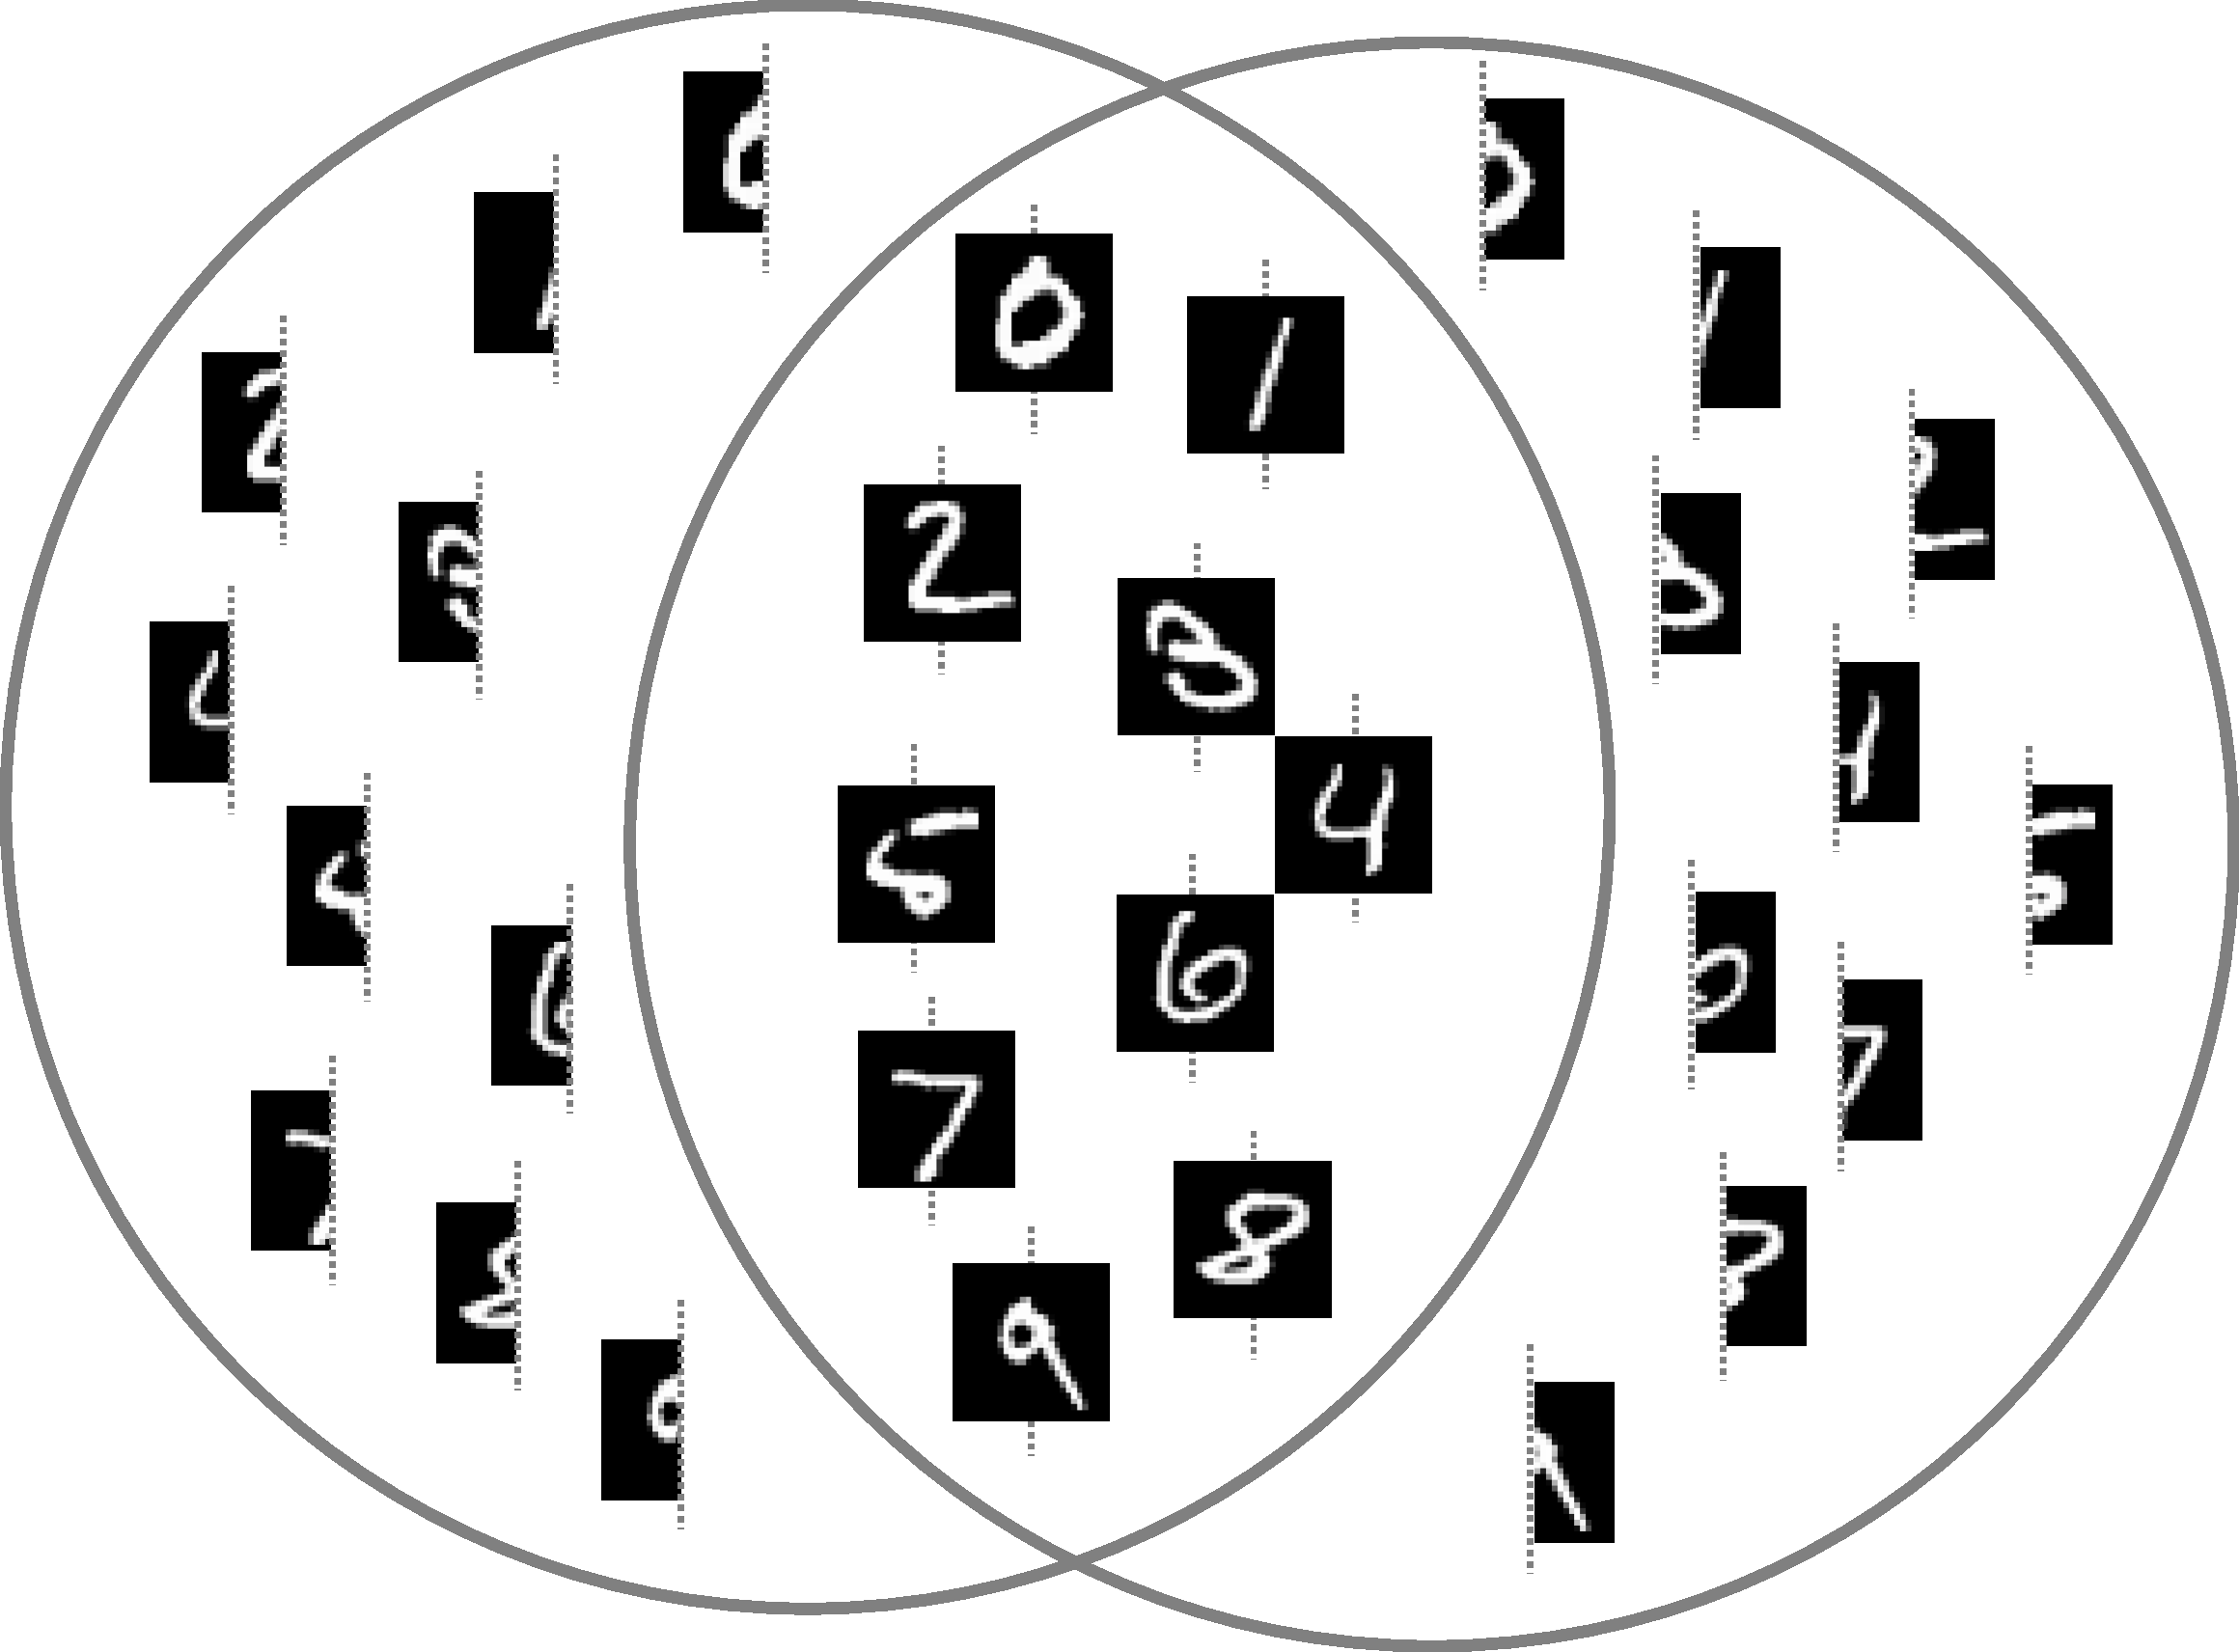
\includegraphics[width=0.8\columnwidth]{./tex/fig/mnist_scheme.pdf}
\caption{
	Pictorial example of training imaging dataset with two views, named \textit{left} and \textit{right} views.
	In this case we have 30 independent observations:
	$10$ with left-views only; $10$ with right-views only; $10$ with complete views.
	The fraction f of observations with complete views is:
	$f = 1/3$.
}
\label{fig:mnist_scheme}
\end{figure}
%
\begin{figure}[!h]
\centering
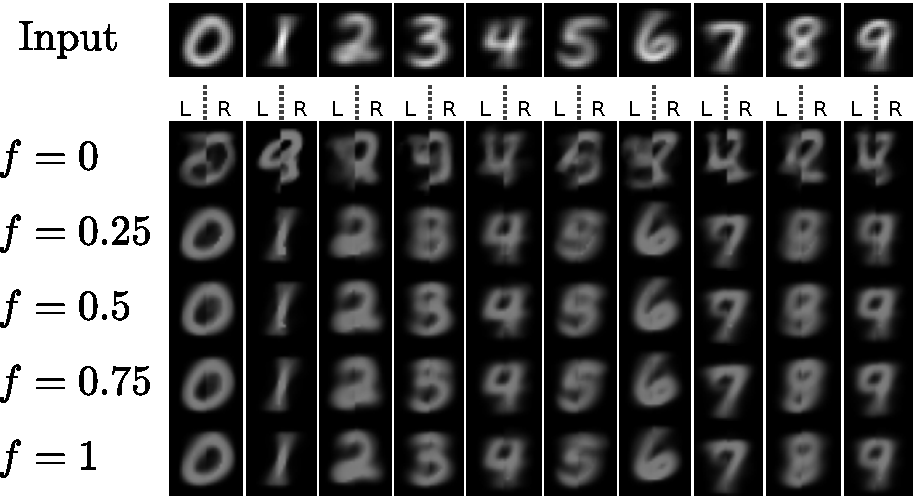
\includegraphics[width=0.8\columnwidth]{./tex/fig/mnist_half.pdf}
\caption{
	Cross reconstruction of digits with increasing degree of data availability ($f$):
	the left side of each digit is inferred from the right side and \textit{vice versa}.
}
\label{fig:mnist_half}
\end{figure}
